\section{The WORG Method}
\label{method}

In order to describe the WORG method, first it is is useful to define  
notation for demand curves and their parameterization.  Call $t$ the time
[years] up to some maximal time $T$ (e.g. 20 years) over which time the
demand curve is know.  Then call $f(t)$ the demand curve, in the natural 
units of the facility type ([GWe] for reactors).
$f(t)$ may be any function that is desired, including non-differential 
functions. For example, though, the demand curve for a 1\% growth rate 
starting at 90 [GWe] has the following form:
\begin{equation}
\label{f-1}
f(t) = 90\times 1.01^t
\end{equation}
Additionally, call $\Theta$ the deployment schedule for the facilities that 
may be constructed to meet the demand.
$\Theta$ is a sequence of $P$ parameters, indexed by $p$, as seen in 
Equation \ref{Theta}.
\begin{equation}
\label{Theta}
\Theta = \left\{\theta_1, \theta_2, \ldots, \theta_P\right\}
\end{equation}
Each $\theta_p$ represents that number of facilities to deploy on its
time step. In simple cases where there is only one type of facility
to deploy $P == T$.  However, when the deployment schedules of multiple 
facility types are needed to meet the same demand curve, $P > T$.  The usual
example for $P > T$ is for transition scenarios which necessarily require 
multiple kinds of reactors.

Now denote $M$ as the sequence for the minimum number of facilities deployable
for the $p$-th deployment. Then call $N$ the sequence of the maximum number
of facilcities deployable. The deployment parameters are thus each defined
on the range $\theta_p \in [M_p, N_p]$. Furthermore, because only whole
numbers of facilities may be deployed $\theta_p \in \N$.  It is also typical, 
but not required for $M = \mathbf{0}$. Zero is also the lower bound
for all possible $\theta_p$ as facilities may not be forcable retired via the
deployment schedule.

From here, call $g(t, \Theta)$ the production as a function of time for a
given deployment schedule. This has the same units as the demand curve.
Thus for power demand and reactor deployments, $g$ is in units of [GWe]. The 
optimization problem can now be posed as an attempt to find a $\Theta$
that minimizes the difference between $f$ and $g$.

\subsection{Dynamic Time Warping}
\label{dtw}

The question of how to take the difference between the demand curve and
the production curve is an important one. The na\"ive option is to simply
take the $L_1$ norm of the difference between these two time series, as
seen in Equation \ref{delta-l1}.  However, since the $g(t, \Theta)$ computed
from a simulation is expensive, any operation that can meaningfully
exacerbate the difference between time series helps drive down the number
of optimization iterations.

Dynamic time warping is just such a mechanism. It computes
a distance between any two time series which compounds the separation
between the two. Additionally, the time series are not required to be of the
same length, though for optimization purposes there is no reason for them
not to be. DTW gives a measure of the amount that one time series would need to
be warped to become the other time series. It is, therefore, a holistic
measure that operates over all times. Dynamic time warping
is more fully covered in \cite{muller}.  However, an
optimization-relevant introduction is given here.

For the time series $f$ and $g$, there are three parts to dynamic time
warping. The first is the distance $d$, which will be minimized. The second
is a cost matrix $C$ that helps compute $d$ by indicating how far a point
on $f$ is from another point on $g$. Thirdly, the warp path $u$ is the
minimal cost curve through the $C$ matrix from the fist point in time to
the last. The DTW distance can thus be interpreted as the
total cost of traveling the warp path.

The first step in computing a dynamic time warp distance is to
assemble the cost matrix. Say that the demand time series $f$ has
length $A$ indexed by $a$, and the production time series $g$ has
length $B$ indexed by $b$. For the optimization problem here, $A$ and $B$
are in practice both equal to $T$.  However, it is useful to have $a$ and
$b$ index the two time series separately. Now denote an $A\times B$ matrix
$\Delta L$ as the $L_1$ norm of the difference between $f$ and $g$:
\begin{equation}
\label{delta-l1}
\Delta L_{a,b} = \left|f(a) - g(b, \Theta)\right|_1
\end{equation}
Since $\Delta L$ uses the $L_1$ norm, $f$ and $g$ may return vector
data. This enables multi-objective optimization. However it is recommended
that the components of the $f$ and $g$ are weighted, normalized, or otherwise
directly comparable.

The cost matrix $C$ may now be defined as the $A\times B$ sized matrix
which follows the recursion relations seen in Equation \ref{cost-matrix}.
\begin{equation}
\label{cost-matrix}
\begin{split}
C_{1,1} & = \Delta L_{1,1}\\
C_{1,b+1} & = \Delta L_{1,b} + C_{1,b}\\
C_{a+1,1} & = \Delta L_{a,1} + C_{a,1}\\
C_{a+1,b+1} & = \Delta L_{a,b} + \min\left[C_{a,b}, C_{a+1,b}, C_{a,b+1}\right]
\end{split}
\end{equation}
The boundary conditions above are the same as setting an infinite cost to
any $a \le 0$ or $b \le 0$. The cost matrix $C$ has the same units as the
demand curve. However, the scale of $C$ is
larger than the demand,
except for in the fiducial case. This is because the cost matrix compounds the
minimum value of previous entries.

Knowing a cost matrix, the warp path can be computed by traversing the
matrix backwards from the $(A, B)$ corner to the $(1, 1)$ corner.
If the length of the warp is $I$ indexed by $i$, the warp path itself
can be thought of as a sequence of coordinate points $u_i$. For a given
point $u_i$ in the warp path, the previous point $u_{i-1}$ may be found by
picking the minimum cost point among the locations one column over $(a,b-1)$,
one row over $(a-1,b)$, and one previous diagonal element to $(a-1,b-1)$.
Equation \ref{warp-path} expresses this mathematically.
\begin{equation}
\label{warp-path}
u_{i-1} = \argmin\left[C_{a-1,b-1}, C_{a-1,b}, C_{a,b-1}\right]
\end{equation}
The maximum possible length of $u$ is thus $\max(I) = A + B$.
The minimum possible length, though, is $\min(I) = \sqrt{A^2 + B^2}$.

The dynamic time warping distance distance $d$ can now be stated as the
cost of the final entry of the warp path normalized by the maximum possible
length of the warp path.
\begin{equation}
\label{d-calc-ab}
d(f, g) = \frac{C_{A,B}}{A + B}
\end{equation}
However, because the demand curve and the production curve
are often defined on the same time grid, $d$ can be further
reduced to the following:
\begin{equation}
\label{d-calc}
d(f, g) = \frac{C_{T,T}}{2T}
\end{equation}
Therefore, $d$ has the same units as the demand curve, production curve,
and cost matrix.

As an example, take a 1\% growth that starts with 90 GWe in the year
2016 as the demand curve. Then consider a production curve that
under-produces the demand by 5\% for 25 years before switching to
over-producing this curve by 5\% for the next 25 years.
Figure \ref{cost-demand-to-production} shows the dynamic time warping
cost matrix between these two time series as a heat map.

\begin{figure}[htb]
\centering
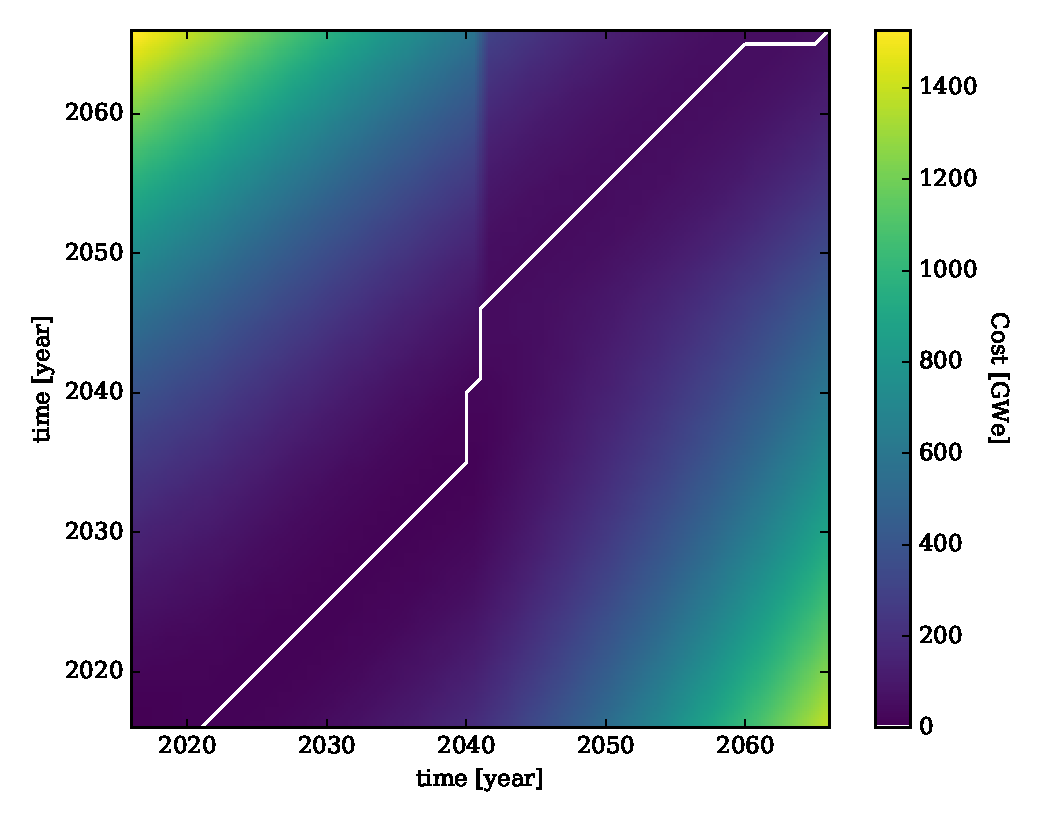
\includegraphics[width=0.9\textwidth]{cost-demand-to-production.eps}
\caption{Heat map of the cost matrix between a 1\% growth demand curve and
a production curve the under produces by 5\% for the first 25 years and then
over produces for the second 25 years.
The warp path $u$ is superimposed as the white curve on top of the
cost matrix.}
\label{cost-demand-to-production}
\end{figure}

Additionally, the warp path between the example demand and production
curves is presented as the white curve on top of the heat map in
Figure \ref{cost-demand-to-production}.
Recognize that $u$ is monotonic along both time axes. Furthermore, the precise
path of $u$ minimizes the cost matrix at every step. Regions of increased
cost in the cost matrix can be seen to repel the warp path. The
distance $d$ between the demand and production curves here happens
to be 0.756 GWe.

Dynamic time warping distance can therefore be used as an objective function
to minimize for any demand and production curves. However, using full
simulations to find $g(t, \Theta)$ remains expensive, even though DTW itself
is computationally cheap. Therefore, a mechanism to reduce the overhead
from production curve evaluation is needed.

\subsection{Gaussian Process Regression}
\label{gp}

Evaluating the production curve for a specific kind of facility using 
full fuel cycle simulations is relatively expensive, even in the 
computationally cheapest case of low-fidelity simulations. This is because a 
fuel cycle realization 
typically computes many features that, though coupled to the production 
curve, are not directly the production curve. For example, the mass balance of 
the fuel cycle physically bounds the electricity production. However, the    
mass balances are not explicitly taken into account when trying to meet
a demand curve.

Alternatively, surrogate models that predict the production curve directly
have many orders-of-magnitude fewer operations by virtue of not computing
implicit physical characteristics. This is not to say that the surrogate 
models are correct.  Rather, they are simply good enough to drive a demand
curve 
optimization. Surrogate models are used here inform a simulator about where
in the parameter space to look next. Truth about production curves should
still be derived from the fuel cycle simulator and not the surrogate model.
In the WORG algorithm, Gaussian processes are used to form the model. 

Gaussian processes are more fully covered elsewhere 
\cite{rasmussen2006gaussian}. Using Gaussian process for optimization has 
also been previously explored \cite{osborne2009gaussian}, though such studies 
tend not to 
investigate the intergal problems posed by facility deployment. As with 
dynamic time warping, a minimal but sufficient introduction to GP is presented 
for the purposes of the deployment optimization.
Conside the case of $Z$ simulations indexed by $z$ that each have a 
$\Theta_z$ deployment schedule and $g_z(t, \Theta_z)$ production curve.

A Gaussian process of these $Z$ simulations is set by its mean and 
covariance functions. The mean function is denoted as $\mu(t, \Theta)$ and 
is the expectation value $\E$ of 
the series of $G$ inputs:
\begin{equation}
\label{G}
G = \left\{g_1(t, \Theta_1), g_2(t, \Theta_2), \ldots, 
           g_Z(t, \Theta_Z)\right\}
\end{equation}
The covariance function is denoted $k(t, \Theta, t^\prime, \Theta^\prime)$ 
and is the expected value of the input to the mean. The mean and 
covariance can be expressed as
in Equations \ref{mean-func} \& \ref{covar-func} respectively.
\begin{equation}
\label{mean-func}
\mu(t, \Theta) = \E G
\end{equation}
\begin{equation}
\label{covar-func}
k(t, \Theta, t^\prime, \Theta^\prime) = 
    \E\left[(g_z(t, \Theta) - \mu(t, \Theta))
            (g_z(t^\prime, \Theta^\prime) - \mu(t^\prime, \Theta^\prime))
      \right]
\end{equation}
Note that in the above, the Gaussian process is itself $P+1$ dimensional, 
since the means and covariance are a function of both the deployment 
schedule ($P$) and time ($+1$).

The Gaussian process $\GP$ approximates the production curve 
given $Z$ simulators. Allow $*$ to indicate that the a quantity comes from 
the model as opposed to coming from the simulator information. A model 
production curve can then be written using either functional or operator
notation, as appropriate:
\begin{equation}
\label{gp-def-approx}
g_*(t, \Theta) \approx \GP\left(\mu(t, \Theta), 
                                 k(t, \Theta, t^\prime, \Theta^\prime)\right) 
                \equiv \GP G
\end{equation}
In machine learning terminology, $G$ serves as the training set for the 
GP model.

Now, when performing a regression on Gaussian processes, 
the nominal functional form for the covariance must be given. 
Such a functional form is also known as the the kernel function.
The kernel contains the \emph{hyperparameters} that are solved for to 
obtained a best-fit Gaussian process. The hyperparameters themselves are
defined based on the definition of the kernel function. Hyperparameter 
values are found via a regression of the maximal likelihood of 
the production curve. Any functional form could potentially serve as a kernel
function. However, a generally useful form is the is the exponential 
squared. This kernel can be seen in Equation \ref{exp2-kernel} with 
hyperparameters $\ell$ and $\sigma^2$ for a vector of parameters $r$:
\begin{equation}
\label{exp2-kernel}
k(r, r^\prime) = \sigma^2 \exp\left[-\frac{1}{2\ell}(r - r^\prime)^2 \right]
\end{equation}
However, other kernels such as the Mat\'ern $3/2$ kernel and Mat\'ern $5/2$
kernel \cite{paciorek2004nonstationary} were observed to be more robust for 
the WORG method. These can be seen in Equations \ref{matern-32} and 
\ref{matern-52} respectively.
\begin{equation}
\label{matern-32}
k(r, r^\prime) = \sigma^2 
                 \left(1 + \frac{\sqrt{3}}{\ell}|r - r^\prime|\right)
                 \exp\left(-\frac{\sqrt{3}}{\ell}|r - r^\prime|\right)
\end{equation}
\begin{equation}
\label{matern-52}
k(r, r^\prime) = \sigma^2 
                 \left(1 + \frac{\sqrt{5}}{\ell}|r - r^\prime|
                         + \frac{5}{3\ell^2}|r - r^\prime|^2\right)
                 \exp\left(-\frac{\sqrt{5}}{\ell}|r - r^\prime|\right)
\end{equation}

From here, say that $\K$ is a covariance matrix 
such that the element at the $r$-th row and $r^\prime$-th column is 
given by whichever kernel is chosen from 
Equations \ref{exp2-kernel}-\ref{matern-52}. Then the 
log likelihood $\log q$ of the obtaining the training set production curves 
$G$ for a given time grid $\mathbf{t}$ and deployment schedule is as 
seen in Equation \ref{log-q}.
\begin{equation}
\label{log-q}
\log q(G|\mathbf{t}, \Theta) 
    = -\frac{1}{2}G^\top\left(\K + \tau^2\I\right)^{-1}G
      -\frac{1}{2}\log\left|\K + \tau^2\I\right|
      -\frac{ZTP}{2}\log 2\pi
\end{equation}
Here, $\tau$ is the uncertainty in the production curves coming from the 
simulations themselves. As most simulators do not report such uncertainties, 
$\tau$ may be set to floating point precision. $\I$ is the usual identity 
matrix. The hyperparameters $\ell$ and $\sigma^2$ are then adjusted via 
standard real-valued optimization methods such that Equation \ref{log-q} is 
minimized. 
This regression of the Gaussian process itself yields the most likely 
model of the production curve, knowing only a limited number simulations.

However, the purpose of such a Gaussian process regression is to evaluate 
the production curve at points in time and for deployment schedules that 
have not been simulated. Take a time grid $\mathbf{t_*}$ and a hypothetical
deployment schedule $\Theta_*$. Now call the covariance vector between
the training set and the model evaluation    
$\mathbf{k}_* = \mathbf{k}(\mathbf{t_*}, \Theta_*)$. 
The production curve predicted by this Gaussian process is then given by
the following:
\begin{equation}
\label{metric-model}
\mathbf{g}_*(\mathbf{t}_*, \Theta_*) = 
    \mathbf{k}_*^\top \left(\K + \tau^2\I\right)^{-1}G
\end{equation}
Equations \ref{mean-func}-\ref{metric-model} are derived and discussed fully
in \cite{rasmussen2006gaussian}. 

However, implementing the above Gaussian process mathematics for the specific
case of the WORG algorithm 
is not needed.  Off-the-shelf Gaussian process modeling software 
libraries already exist and are applicable to the regression problem here.
Scikit-learn v0.17 \cite{scikit-learn} and George v0.2.1 \cite{hodlr} 
implement such a method and have a Python interface. George is specialized 
around Gaussian processes, and thus is preferred for WORG over scikit-learn, 
which is a general purpose machine learning library.

As an example, consider a Gaussian process between two power production 
curves similar to the example used in \S\ref{dtw}. The first is a nominal 1\% growth 
in GWe for 50 years starting at 
90 GWe in 2016. The second curve under produces the first curve by 10\% 
for the first 25 years and over produces by 10\% for the last 25 years.
Additionally, assume that there is a 10\% error on the training data set.
This will produce a model of the mean and covariance that splits the 
difference between these two curves. This example may be seen graphically
in Figure \ref{gwe-model-}.

\begin{figure}[htb]
\centering
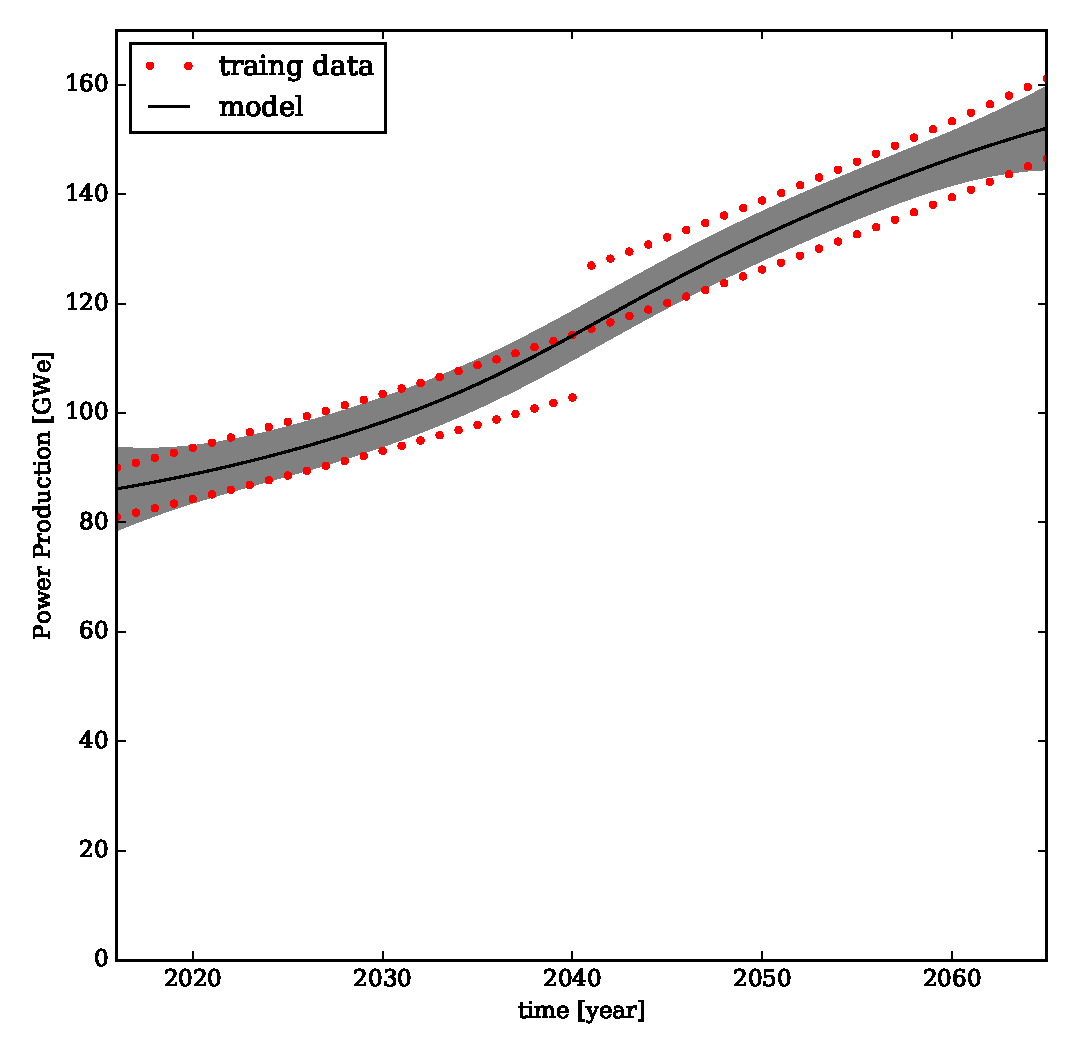
\includegraphics[width=0.9\textwidth]{gwe-model-.eps}
\caption{The Gaussian process model of a 1\% growth curve along with the
an initial 10\% under production followed by a 10\% under production. 
The model is represented by the black line that runs between the red 
training points. Two standard deviations form the model are displayed as the
gray region.}
\label{gwe-model-}
\end{figure}

The simple example above does not take advantage of an important 
feature of Gaussian processes. Namely, it is not limited to two production
curves in the training set.  As many as desirable may be used.  This will
allow the WORG algorithm to dynamically adjust the number of $Z$ simulations 
which are used to predict the next deployment schedule. WORG is thus capabale
of 
effortlessly expanding $Z$ when new and useful simulations yield valuable production
curves.  However, it also enables $Z$ to contract to discard production
curves that would drive the deployment schedule away from an optimum.

Now that the Gaussian process regression and dynamic time warping tools have 
been added to the toolbox, the architecture of the WORG algorithm can 
itself be described.

\clearpage

\subsection{WORG Algorithm}
\label{algo}

The WORG algorithm has two fundemantal phases on each iteration:
estimation and simulation.  These are preceded by an initialization 
before the optimization loop. Additionally, each iteration decides 
which information from the previous simulations is worth keeping for the
next estimation. Furthermore, the method of estimating deployment 
schedules may be altered each iteration.  Listing \ref{worg-pseudo}
shows the WORG algorithm as Python pseudo-code. A detailed walk-through 
explination of this code will now be presented.

Begin by initializing three empty sequences $\vec{\Theta}$, $G$, and $D$.
Each element of these series represents deployment schedule $\Theta$, 
a production curve $g(t, \Theta)$, and a dynamic time warping history 
between the demand and production curves $d(f, g)$ as seen previously.
Importantly, $\vec{\Theta}$, $G$, and $D$ only contain values for
the relevant optimization window. For example, root finding algorithms
such as Newton's method and the bisection method have a lenght-2 window
since they use the $(s-1)^\mathrm{th}$ point and the $s^\mathrm{th}$ point
to compute the $(s+1)^\mathrm{th}$ point. Since a Gaussian process model is 
formed, any or all of the $s$ iteration information may be used. However, 
Allowing the time window to be either two or three depending on the 
circumstances balances the need to keep the points with the lowest $d$ 
values while pushing the model far from known regions with higher 
dinatnces. WORG effectively tries to have $D$ contain one high-value $d$
and one or two low valued $d$ at all iterations. 

To this end, $\vec{\Theta}$, $G$, and $D$ are initialized with two 
bounding cases. The first is to set the deployment schedule equal to the
lower bound of the number of deployments $M$.  Recall that this is 
usually $\mathbf{0}$ everywhere, unless a minimum number of facilities 
must be deployed at a specific point in time. Running a simulation with 
$M$ will then yeild a production curve $g(f, g)$ and the DTW distance to
this curve.  Note that just because the no facilites are deployed, the 
production curve need not be zero due to the initial conditions of the 
simulation, where existing facilities will continue to produce. 

Similarly, another simulation may be executed for the maximum possible
deployment schedule $N$. This will also provide information on the 
production over time and the distance to the demand curve. $M$ and $N$
form the first two simulations, and therefore the loop 
variable $s$ is set to two.

\clearpage
\begin{lstlisting}[
    caption={WORG Algorithm in Python Pseudo-code},
    label=worg-pseudo,mathescape]
Thetas, G, D = [], [], []  # initialize history

# run lower bound simulation
g, d = run_sim(M, f)
Thetas.append(M)
G.append(g)
D.append(d)

# run upper bound simulation    
g, d = run_sim(N, f)
Thetas.append(N)
G.append(g)
D.append(d)

s = 2
while MAX_D < D[-1] and s <= S:
    # set estimation method
    method = initial_method
    if method == 'all' and (s%4 < 2):
        method = 'stochastic'

    # estimate deployment schedule and run simulation
    Theta = estimate(Thetas, G, f, method)
    g, d = run_sim(Theta, f)
    Thetas.append(Theta)
    G.append(g)
    D.append(d)

    # take only the most important and most recent schedules
    idx = argsort(D)[:2]
    if D[-1] == max(D):
        idx.append(-1)
    Thetas = [Thetas[i] for i in idx]
    G = [G[i] for i in idx]
    D = [D[i] for i in idx]
    s = (s + 1)
\end{lstlisting}
\clearpage

The optimization loop may now be entered.  This loop has two conditions.
The first is that the next iteration occurs only if the last distnace
is greater than a threshold value $\mathrm{MAX\_D}$. The second is that 
the loop variable $s$ must be less than or equal the maximum number
of iteration $S$.

The first step in each iteration is to choose the estimation method. The
three mechanisms will be discussed in detail in \S\ref{selecting}. For
the purposes of the optimization loop, they may be represented by the 
\stochastic, \innerprod, and \allflag flags. The stochastic method 
chooses many random deployment schedules to test. Alternatively, an inner
product of search of the space defined my $N$ and $M$ may be performed. 
Lastly, the \allflag performs both of the previous estimates and takes
the one with lowest computed distance.  However, \allflag can sometimes
declare the inner product the winner for all $s$.  This can itself 
be problematic since this estimation method has the tendancy to form 
deterministic loops when close to an optimimum. This behavior is not unlike
simliar loops formed with floating point approximations to Newton's method.
To prevent this when using \allflag, WORG forces the stochastic method
for two consecutive iterations out of every four.  
 
A best-guess estimate for a deployment schedule $\Theta$ is finally 
made.  This takes the previous deployment schedules $\vec{\Theta}$ and
production curves $G$ and forms a Gaussian process model. Potential 
values for $\Theta$ are explored according to the method provide.  The 
$\Theta$ that produces the minimum dynamic time warping distance between
the demand curve and the model $d(f, g_*)$ is then returned.

The $\Theta$ estimate is then supplied to the the simulator itself and 
a simulation is executed.  The details of this prcedure are, of course,
simulator specific.  However, the simulation combined with any post-processing 
needed should return an aggregate production curve $g_s(t, \Theta)$.  
This is then compared to demand curve via $d(f, g_s)$. After the simulation, 
$\Theta$, $g_s(t, \Theta)$, and $d(f, g_s)$ are appended to the 
$\vec{\Theta}$, $G$, and $D$ sequences.  Importantly, note that the 
production curve and DTW distance from the simulator are appended, 
not the production curve and distance from the estimate model.

Concluding the optimization loop, $\vec{\Theta}$, $G$, $D$, and $s$ are
updated.  This begins by finding and keeping the two elements with the 
lowest distances between the demand and production curves.  However, 
if the most recent simualtion yeilded the largest distance, this is also
kept for the next iteration. Keeping the largest distance serves to deter
exploration in the direction on the next iteration.  Thus a sequence of 
two or three indices is chosen. These indices are applied to redefine
$\vec{\Theta}$, $G$, and $D$. Lastly, $s$ is incremented by one and the
next iteration begins.

The WORG algorithm presented here shows the overall structure of the 
optimization.  However, equally important and not covered here is how the
estimation phase chooses $\Theta$.  The methods that WORG may use are 
presented in the following sections, which rounds out the methodology. 
